\documentclass[../Head/Main.tex]{subfiles}
\begin{document}
\section{SORA Assessment}
\subsection{Step 1: Concept of Operations}
The operation consists of a drone provided by SDU employed for fence inspection at the perimeter of HCA Airport. The operation is fully autonomous with a pilot in-charge of monitoring the UAV during all stages of take-off, landing and inspection. The operation will be expectedly carried out 3 time a day.
\subsubsection*{A1.3 Type of operations:}
The type of operation is visual line of sight (VLOS) as the pilot in-charge of the drone needs to monitor and control all the phases of drone operation. The operation is carried out in sparsely populated area of Beldringe Odense Denmark. The airspace is in the vicinity of an active small-scale airport in a fully integrated airspace.
\begin{itemize}
    \item Maximum Flight height : 20 m \vspace{-5pt}
    \item Inspection height : 1-2.5 m \vspace{-5pt}
    \item Contingency volume : 50 m in all directions \vspace{-5pt}
    \item Ground Risk Buffer : 100 m (Due to vicinity of airport buildings) \vspace{-5pt}
    \item Air Risk Buffer : 100 m (Due to fence being in vicinity of the runway)
\end{itemize}
\begin{figure}[H]
    \centering
    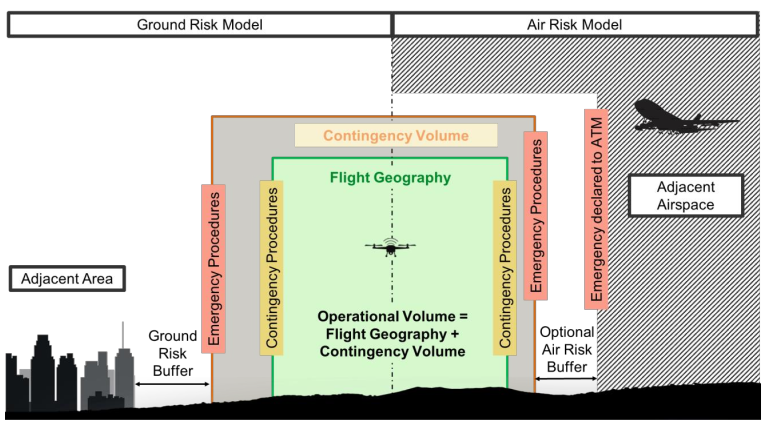
\includegraphics[width=0.5\textwidth]{../Figures/buffer.png}
    \caption{UAV Ground and Air Risk Model\cite{sora_doc}}
    \label{fig:sora_buff}
\end{figure}
\vspace{-10pt}
\subsubsection*{A.1.3.2 Normal operation strategy:}
The operation is normally carried out by a certified drone pilot and the complete operation is owned by the airport authority of HCA Airport. The operator is expected to conduct inspection for 3 times a day maximum. Since the operation is done on behalf of airport authorities the pilot is in contact with the control tower for any coordination regarding incoming and outgoing traffic at HCA.
\subsubsection*{A1.4 Remote crew training:}
The pilot in-charge for operating the drone is trained to intervene in case of any failure and deviation from standard inspection path of the drone.
\subsubsection*{A2.2 UAS Description:}
\begin{table}[H]
\centering
\caption{UAV Technical Specifications}
\label{tab:my-table}
\begin{tabular}{|l|l|}
\hline
\textbf{Weight}   & 2500 g               \\ \hline
\textbf{WxLxH}    & 578 x 578 x 330 mm   \\ \hline
\textbf{Wingspan} & 832 mm               \\ \hline
\textbf{Material} & Plastic/carbon fiber \\ \hline
\textbf{Airframe} & Hexacopter           \\ \hline
\end{tabular}
\end{table}


\begin{table}[H]
\centering
\caption{UAV Operational Specifications}
\label{tab:my-table}
\begin{tabular}{|l|l|}
\hline
\textbf{Endurance}             & 19 min    \\ \hline
\textbf{Payload capacity}      & 700 g     \\ \hline
\textbf{MTOW}                  & 3200 g    \\ \hline
\textbf{Operating temperature} & 5 - 45 °C \\ \hline
\end{tabular}
\end{table}

\underline{Sensors}: The drones sensors comprises of IMU, GPS and Intel RealSense D435 camera.

\subsubsection*{A.2.3 UAS control segment:}
\underline{Navigation}: The drone uses PX4 flight controller which uses GPS for location and navigation. The secondary means of navigation is manual operation of the drone by the remote pilot. In case of navigation system failure, the flight termination system will activate and try to land the drone using IMU feedback. The drone pilot is also expected to intervene in case such failure occurs. In normal operation, the route is pre-processed and uploaded as a mission to the drone.

\subsubsection*{A.2.4 Containment system:}
In case of the drone deviating from the intended route the pilot is trained to act and take control of the drone to bring it back in the intended operating area or terminate the operation by deploying the flight termination system.

\subsubsection*{A.2.6 Command and control (C2) link segment:}
The communication with UAV is a telemetry link and RC controller link. In case of the failure of these links the UAV will enter in a fail safe mode and initiate landing. Furthermore, in the future another communication link provided by Lorenz Technology called AI Link, which could further reduce the chances of communication failure with the drone.

\subsubsection*{A.2.9. Safety features:}
The drone has all the safety features inherent in PX4 flight controller. In addition to this the monitoring by the remote pilot makes sure that the drone is operating as intended.


\subsection{Step 2: Determination of the intrinsic UAS ground risk class (GRC)}
The maximum dimension of the drone is 578 mm, maximums speed is 5 m/s and the maximum weight is 3200 g. This gives us an estimate of the typical kinetic energy of the drone: 40 J.

\[ KE = 1/2 m\cdot v^2 = 40 J \]

Also the type of operation is VLOS over a ground area which gives us the \textbf{Intrinsic Ground Risk Class of 1} according to table 2 Annex I of the document. \cite{sora_doc}

\subsection{Step 3: Final GRC determination}

The primary mitigation strategy for Ground Collision Risk is active monitoring by the drone pilot. Since the drone is flying at quite low speed 0.5-1.0 m/s at the height of 1-2 meter above ground in a sparsely populated area the need for mitigation of ground risk is deemed unnecessary.
The final GRC is determined as below:
\begin{itemize}
\item M1: 0 (No strategic mitigation)
\item M2: 0 (No mitigation for ground impact)
\item M3: 0 (ERP in the form of operator takeover in case of drone malfunction)
\end{itemize}
Final GRC  index is 1 + (0+0+0) = 1

\subsection{Step 4: Determination of the initial air risk class (ARC)}
The operation is carried out in Flight level less than 500ft AGL in the vicinity of the small-scale operational airport. Therefore, according to figure 4 of the document \cite{sora_doc}) the initial ARC of the operation is determined to be ARC-d.

\subsection{Step 6: TMPR (Tactical mitigation performance requirements) and robustness levels}
In this step, we determine the tactical mitigation required to mitigate the air risk class identified in the previous step. Since the operation is always done in VLOS mode with active monitoring of the drone by the pilot, it is considered as sufficient means of compliance for mitigating the risk of air collision. The tactical mitigation during the fence inspection drone operation is:
\begin{itemize}
    \item Operation in VLOS to avoid any manned air traffic
    \item Active collaboration with HCA tower controller during the operation where the operation is paused in case of any incoming/outgoing traffic.
    
\end{itemize}
These TMPR (Tactical Mitigation performance requirements) are satisfactory for the operational scenario.
\subsection{Step 7: SAIL determination}
\begin{figure}[H]
    \centering
    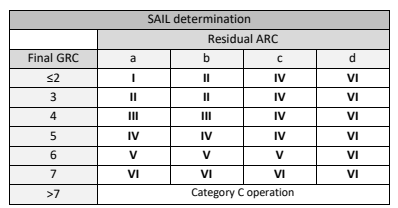
\includegraphics[width = 0.5\textwidth]{../Figures/sail.png}
    \caption{SAIL Determination Chart}
    \label{fig:sora_sail}
\end{figure}
Residual GRC : 1 \\
Residual ARC : d \\
SAIL : VI \\

The SAIL parameter is the consolidated measure of GRC and ARC  and demonstrates the level of confidence that the operation will be under control. It further specifies which OSOs (Operational Safety Objectives) will be required for the operation.

\subsection{Step 8: Identification of operational safety objectives (OSOs)}
The following OSOs are required to be complied with for the operation of the fence inspection drone:
%%%%%%%%%%%%%%%%%%%%%%%%%%%%%%%%%%%%%%%%%%
Table attached in Appendix \ref{tab:sora_oso}
%%%%%%%%%%%%%%%%%%%%%%%%%%%%%%%%%%%%%%%%%%

\subsection{Step 9: Adjacent Area/Airspace considerations}
Since the drone is being operated in the vicinity of an operational airport, the complete operation has been designed and developed keeping the airspace considerations in mind.


\end{document}